\documentclass[letterpaper, 12pt]{article}
\usepackage{graphicx}
\graphicspath{ {pictures/} }
\usepackage{listings}
\usepackage[pdf]{pstricks}
\usepackage{pst-optexp}

\setlength{\parskip}{1em}

\title{Modern Physics Laser Scanning Project}
\author{Alvin Lin
  \thanks{with Jion Fairchild and Sachal Malick}}
\date{June 2016}

\begin{document}

\begin{titlepage}
\maketitle
\end{titlepage}

\begin{abstract}
This experiment was conducted in the Modern Physics class of 2016 at Stuyvesant High School. The goal was to build a laser scanner using a laser and a photodiode and find the maximum achievable resolution of the apparatus.
\end{abstract}

\section{Experimental Setup}
\par
In this experiment, we focused a laser onto a piece of paper containing our
scanning sample and read the amount of reflected light using a photometer. The photometer displayed the amount of light it received on a digital display but also conveniently had two banana jacks that outputted a voltage linearly proportional to the amount of light it received. This allowed us to connect an Arduino microcontroller to the photometer to read and store the voltages as we passed the scanning sample beneath the laser. We 3D printed two important parts to our scanner, the slides for the x and y axes.
\par
In order to maximize the resolution of our image, we wanted the laser beam to be as small and as focused as possible. We spaced three concave lenses in front of the laser to expand the beam, collimate it, and focus it to a point. The scanning sample would be placed at the end of the focused beam. If the laser was focused on a darker point on the sample, it would reflect less light. Conversely, if the laser was focused on a lighter point, it would reflect more light.

\begin{pspicture}[](0,0)(14,4)
  \pnodes(2,2){A}(12,2){B}
  \pnodes(10.5,1.5){D}(10.7,2){E}(10.9,2.5){F}
  \begin{optexp}
    \optbox[position=start](A)(B){laser}
    \lens[lensradius=0.75,abspos=1,labeloffset=-1](A)(B){expands beam}
    \lens[lensradius=2.3,abspos=4](A)(B){collimates beam}
    \lens[lensradius=0.75,abspos=8](A)(B){focuses beam}
    \mirror[labeloffset=-0.7](D)(E)(F){sample}
    \drawwidebeam[beamwidth=0.2,linecolor=red]{-}(B)
  \end{optexp}
\end{pspicture}

\par
We built our own 2D slide mechanism to shift the scanning sample back and forth under the laser. We used an Arduino to read the voltage output from the photometer and simultaneously control two stepper motors which would shift the sample back and forth.

\begin{figure}
  \centering
  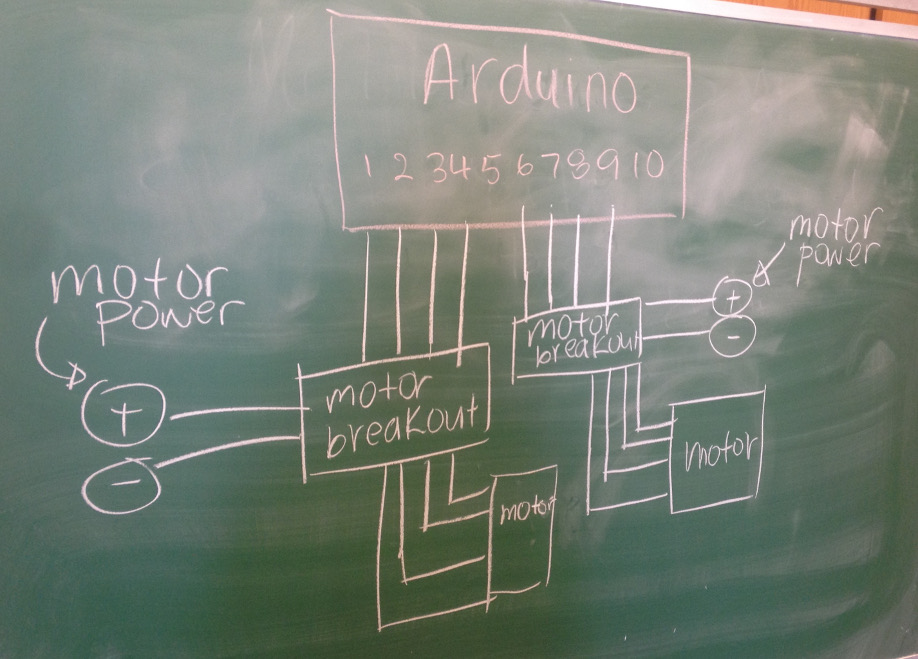
\includegraphics[width=12cm,height=9cm]{circuit}
  \caption{Diagram of Components}
\end{figure}

\begin{figure}
  \centering
  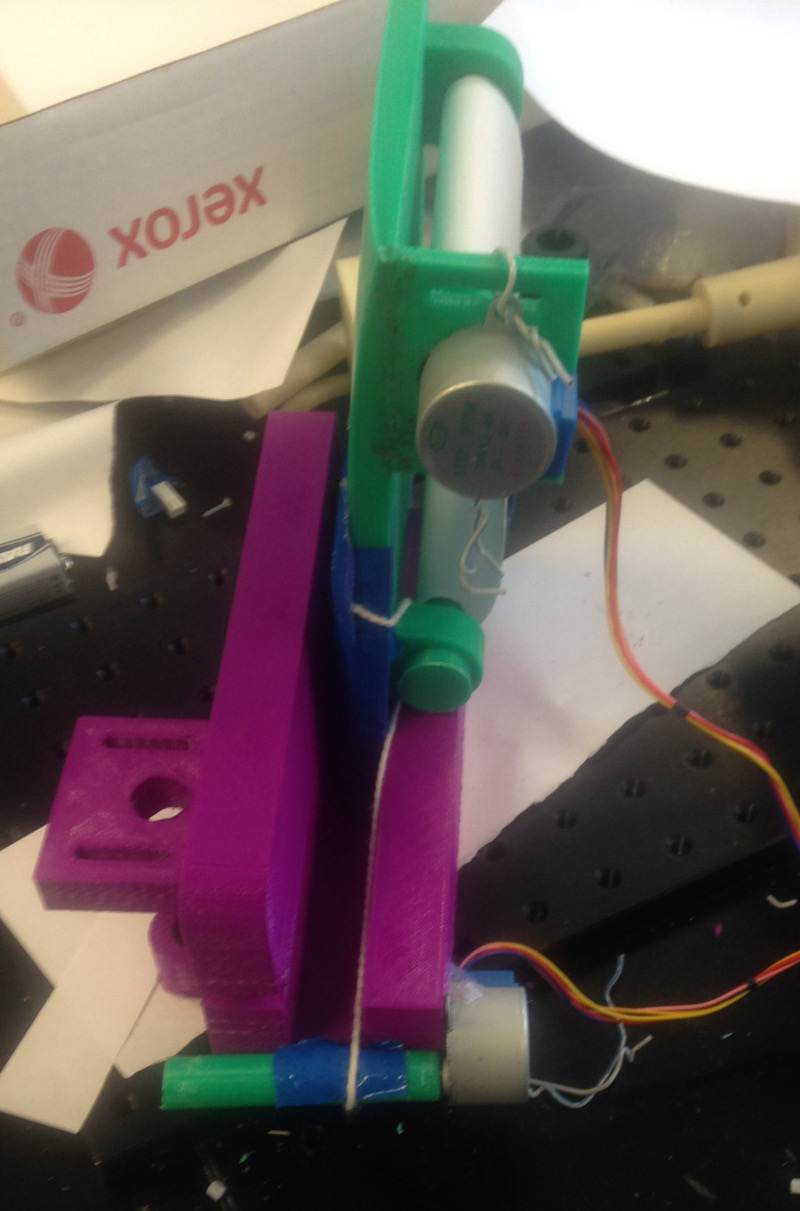
\includegraphics[width=9cm,height=12cm]{setup}
  \caption[caption]{3D printed components, CADs available here:\hspace{\textwidth}https://www.github.com/omgimanerd/im-firing-my-lazer}
\end{figure}

\section{Experimental Procedure}
\par
We set up various resolution test targets beneath our scanner and ran our scanner over each target. Based on the stepper motors and driver boards we were using\footnotemark, we approximated what the resolution of our setup would be.
\footnotetext{We were using the USPRO 5V 4-phase 5-wire stepper motors with the ULN2003 driver board for Arduino}
Due to the driver board's microstepping, each revolution of the motor took 2048 steps. With a 0.5 inch diameter drive axle moving the sample, this means that 1 step equated to \( 7.6699 \times 10^{-4} \) inches. Converting this to \( \frac{lines}{mm}\):

\[ 7.6699\times10^{-4}in = 1.9557746\times10^{-2}mm \]
\[ \frac{1\ line}{1.9557746\times10^{-2}mm} = 51.13\frac{lines}{mm}\]
\[ 51.13\frac{lines}{mm} \div 2 \approx 25\frac{lines}{mm} \]

\par
This number is only true, however, if our laser beam is an infinitesimally small point. Since this is not the case, our actual resolution is much lower.


\end{document}
